\documentclass[a4paper,12pt]{article}
\usepackage{polski}
\usepackage[utf8]{inputenc}
\usepackage{graphicx}
\title{Dźwięk i muzyka w systemach komputerowych. Synteza addytywna. Lab 08}
\author{Marcin Fabrykowski}
\date{}
\begin{document}
\maketitle
\newpage
Celem ćwiczenia jest zbudowania syntezatora addytywnego przy pomocy programu SynthEdit.\\
Zadanie to obrazuje poniższy schemat
\begin{figure}[h]
\hspace{-3.5cm}
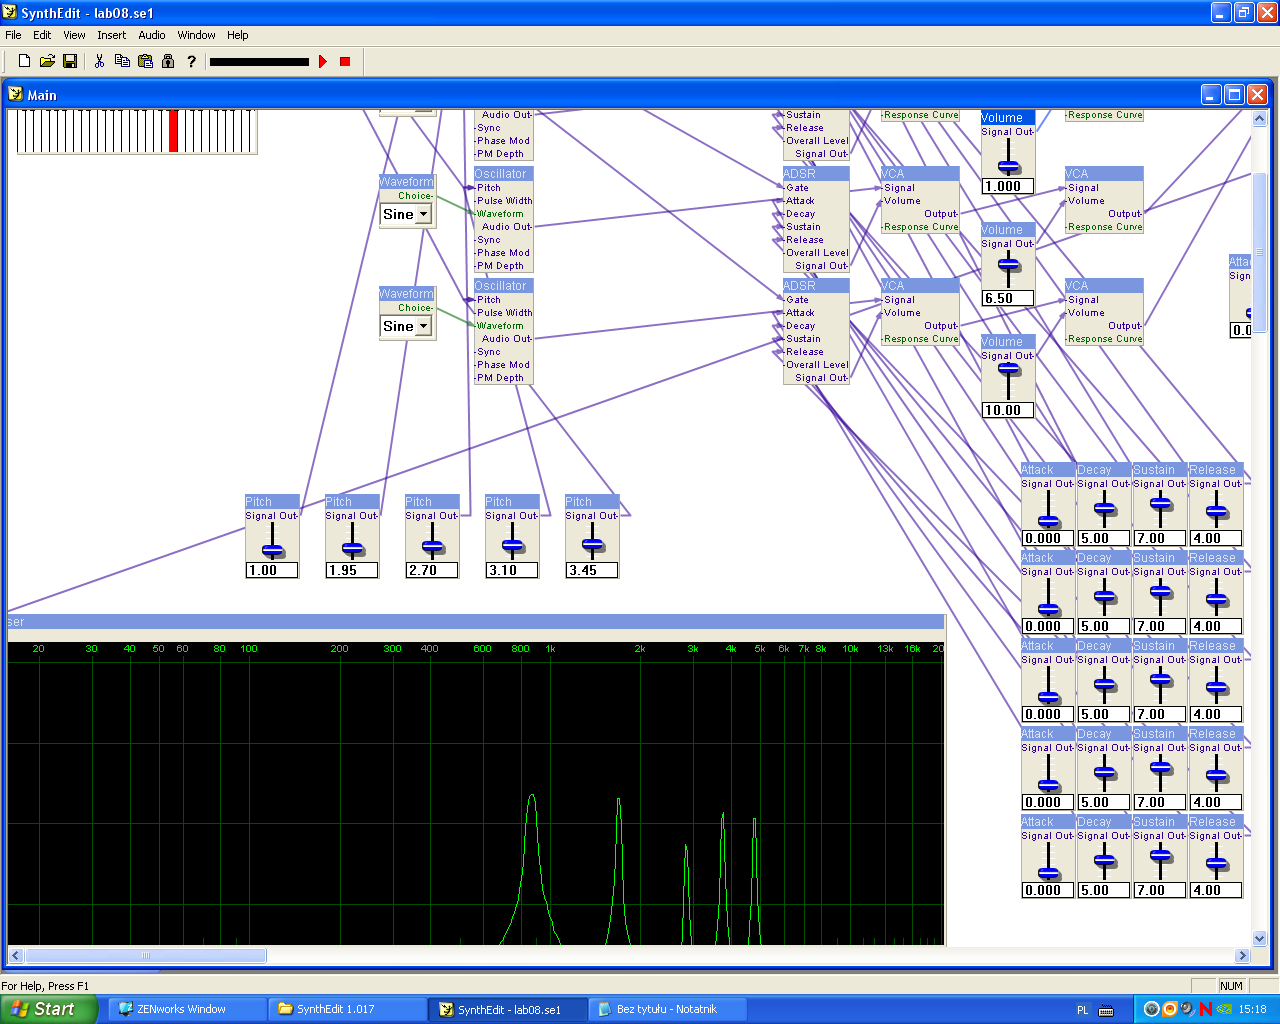
\includegraphics[scale=0.45]{lab08.png}
\end{figure}
\end{document}

